\chapter{Baggrund}

\section{Hjertet}
Hjertet, \textit{cor}, er en hul muskel, der har til opgave at pumpe blodet rundt til hele kroppen. Hjertet består af i alt fire kamre. To forkamre, atrier, og to hjertekamre, ventrikler. Atrierne fungere primært som reservoir for blod, mens ventriklerne fungerer som den effektive pumpe.\\

\begin{figure}[htb]
	\centering
	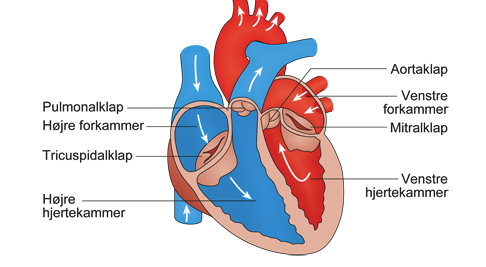
\includegraphics[width=1\textwidth]{Figurer/Snip20150410_31}
	\caption{Hjerte med forklarende pile \protect\footnotemark} 
\end{figure}
\footnotetext{Billede fra Hjerteforeningens hjemmeside.\textbf{Indsæt hyperlink - ligger i en note på Lises computer}}

Hjertekamrene og forkamrene er adskilt fra hinanden af anulus fibrosus, som er en plade af bindevæv. Anulus fibrosus består af fire bindevævsringe, der er forbundet med hinanden. To af disse udgør åbningerne mellem atrierne og ventriklerne. De to sidste danner åbningerne mellem højre hjertekammer og lungepulsåren og venstre ventrikel og hovedpulsåren. Ved alle bindevævsringene er der klapper, der fungere som ventiler.\\ 
AV-klapperne \textbf{ORDLISTE, atrioventrikulær - klapperne} sidder mellem atrierne og ventriklerne. Klappen mellem højre atrier og ventrikel kaldes tricuspidalklap, mens klappen mellem venstre atrier og ventrikel kaldes mitralklap. Aortaklappen er placeret ved afgangen af hovedpulsåren og pulmonalklappen ved afgangen af lungepulsåren. Klapperne fungere således, at blodet kun kan løbe én vej gennem dem. Åbningen samt lukningen af disse er en passiv proces, som bestemmes af forskelle i væsketrykket på de to sider af klapperne.\\ 

\begin{figure}[htb]
	\centering
	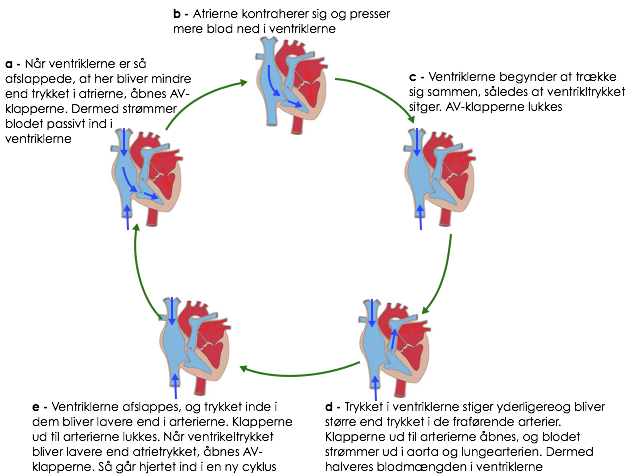
\includegraphics[width=1\textwidth]{Figurer/Snip20150412_7}
	\caption{De forskellige faser i hjertets cyklus \protect\footnotemark}
\end{figure}
\footnotetext{Billede fra "Menneskets anatomi og fysiologi" s. 273 figur 9.6}

Hjertets cyklus inddeles i to hovedfaser. Den første kaldes diastolen. I diastolen er ventriklerne afslappede og fyldes med blod. Det vil sige, at trykket i ventriklerne bliver lavere end trykket i atrierne, således at AV-klapperne åbnes, og blodet begynder at strømme ind i ventriklerne. Under hele diastolen er aortaklappen lukket. Den anden fase kaldes systolen. I systolen kontraherer ventriklerne sig. Trykket i ventriklerne overstiger trykket i atrierne, således at AV-klapperne lukkes, så tilbagestrømning af blod til atrierne forhindres. Når ventriklerne har kontraheret sig så meget, at trykket i ventriklerne overstiger trykket i hovedpulsåren samt i lungepulsåren, åbnes aortaklappen og pulmonalklappen, og blodet strømmer ud i hovedpulsåren og lungepulsåren. Ventriklernes tryk falder igen til under atriernes tryk, hvilket påvirker at AV-klapperne åbnes igen og diastolen begynder igen.\\
Hjertets cyklus igangsættes i sinusknuden ved aktionspotentialer, der føres til de forskellige dele af hjertet. Dette sker enten ved, at aktionspotentialet går fra hjertemuskelcelle til hjertemuskelcelle gennem åbne celleforbindelser. Eller gennem åbne celleforbindelser mellem specialiserede hjertemuskelceller i hjertets specielle ledningssystem. Det specielle ledningssystem består af tre sammenhængende dele - AV-knuden \textbf{ Ordliste}, det hiske bundt gennem anulus fibrosus og det hiske bundt over i purkinjefibrene \textbf{ ordliste}. \\
Hjertets ledningssystem har to hovedopgaver. Først at sørge for, at aktionspotentialet spredes hurtigt gennem hjertet, og dermed sørge for al hjertemuskulaturen i ventriklen kontraheres næsten samtidig. Denne næsten samtidige kontraktion medfører, at der inde i ventriklerne opbygges et effektivt tryk. Purkinje fibrene, som kun er i ventriklerne og ikke atrierne, gør at aktionspotentialerne spredes hurtigere i ventriklerne end i atrierne. Den anden hovedopgave er derfor at sørge for en vis forsinkelse i impulsledning fra atrierne til ventriklerne. Forsinkelsen er mulig, da anulus fibrosus, der adskiller atrierne og ventriklerne, fungerer som en elektrisk isolator. Derfor skal aktionspotentialet ledes fra atrierne til ventriklerne via det specialiserede ledningssystem, og da AV-knuden leder aktionspotentialet særlig langsomt, opstår forsinkelsen. Dette medfører, at atriernes kontraktion fuldføres, før ventriklernes igangsættes, dermed er der sikret en tilstrækkelig fyldning af ventriklerne, før de pumper blodet videre. Denne spredning og udløsning af aktionspotentiale sker regelmæssigt, og er den afgørende faktor for hjertets kontraktions rytme.
\begin{figure}[htb]

	\centering	
	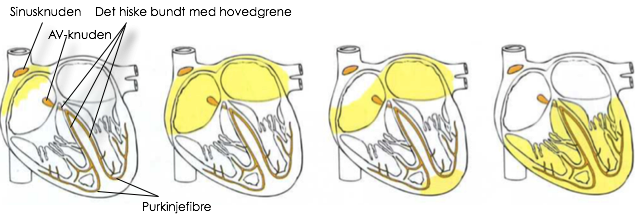
\includegraphics[width=1\textwidth]{Figurer/Snip20150410_6}
	\caption{Spredning af aktionspotentialer gennem hjertet \protect\footnotemark}
\end{figure}
\footnotetext{"Menneskets anatomi og fysiologi" s. 275 figur 9.9}

I \textit{Figur 3.3} ses spredningen af aktionspotentialer gennem hjertet. Aktionspotentialet udløses i sinusknuden og forsinkes i AV-knuden. Dernæst ledes aktionspotentialet videre til ventrikelmuskulaturen. De farvelagte områder er de depolariserede områder og det ses, at atriernes depolarisering er afsluttet før ventriklernes er startet.

\section{Elektrokardiogram}
Et elektrokardiogram, EKG, afspejler hjertets elektriske aktivitet. Teknikken kaldes elektrokardiografi og udføres via elektroder, der er placeret forskellige steder på kroppen, primær omkring hjertet. Elektroderne måler den elektriske aktivitet via en overflade strøm, der går ud fra thorax. Det er disse strømme, som danner de forskellige graf-udsving, som er EKG-signalets takker. Takkerne viser atriernes- og ventriklernes systole og diastole, og er inddelt i P-takken, QRS-komplekset og T-takken. \\
P-takken viser atriets depolarisering, \textbf{og dertil er der P-takken til QRS-komplekset, der er aktionspotentialet fra atrier til ventrikler.} QRS-komplekset udgør tilsammen ventrikel depolarisering. QRS-komplekset er større end P-takken, da muskelmassen i ventriklerne er større end atriernes muskelmasse, hvilket påvirker en højere elektrisk aktivitet. T-takken beskriver ventriklernes repolarisering. Denne er også mindre end QRS-komplekset, da repolariseringen forløber langsommere end depolariseringen.\\
Elektrokardiografi giver et billede på, hvordan ens hjerte fungere. Nedenfor ses et EKG-signal for et raskt hjerte. Hvis ens hjerte ikke fungere optimalt, vil ens EKG-signal se anderledes ud og en sundhedsfaglig person vil kunne diagnosticere patienten ud fra grafen.  En patient kunne have atrieflimmer, som er den sygdom, dette projekt handler om.  

\begin{figure}[htb]
	\centering
	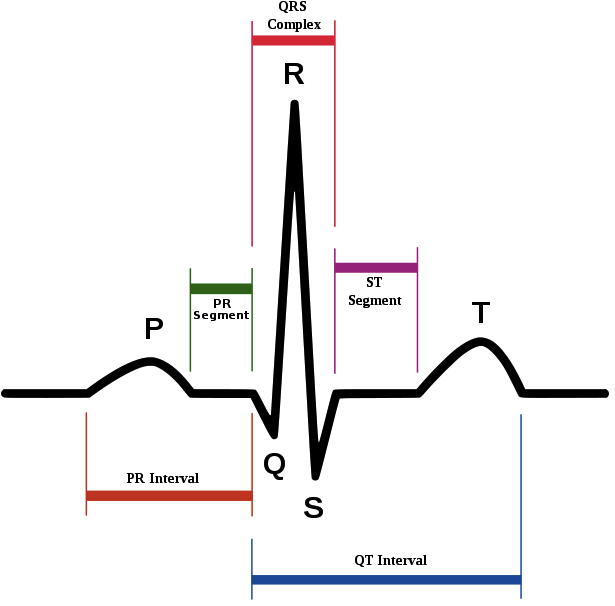
\includegraphics[width=1\textwidth]{Figurer/Snip20150412_36}
	\caption{Normalt EKG-signal}
\end{figure}


\section{Atrieflimren}
Atrieflimren forekommer, når atrierne ikke kontraherer sig ordentligt. Den hyppigste udløsning af atrieflimren forefalder pga. en serie af hurtige impulser (ekstrasystoler).  De kommer fra den atriemuskulatur, som sidder nær lungevenerne i venstre atrium \textbf{er det det samme som artie??} . Dermed bliver atriernes normale kontraktionsmønster ødelagt, og de begynder at "flimre". Under atrieflimren fungerer sinusknuden stadig som normalt, men har ingen kontakt til atrium.\\
Pga. arytmien mister man den regelmæssige atrietømning og en får nedsat funktion af hjertets pumpningen. Blodet vil ophobe sig i atriet og danne lokale tromber.  De kan løsrive sig og flyde med blodstrømmen ud i kroppen, hvor de kan sætte sig fast (embolisere). Ubehandlet emboliserende atrieflimren er årsagen til 1/3 af alle cerebral apopleksiske tilfælde. Derfor er det vigtigt at være opmærksom på tilstedeværelse af atrieflimren hos netop disse indlagte patienter.\\
Hvis arytmien står på i længere tid, og ventrikelfrekvensen er hurtig, kan det udløse hjerteinsufficiens med tiltagende dilatation og dårlig kontraktion af ventriklerne. \\
Atrieflimren opstår som anfald (paroksystisk), der spontant konverterer til normal sinusrytme efter få timer eller dage. Med årerne bliver arytmien mere vedvarende (persisterende) for til sidst at blive kronisk.  De symptomer som kan forbindes med atrieflimren er en øget træthed, åndenød og en forhøjet samt uregelmæssig puls, der kan være utydelig og hurtig. Desuden vil blodtrykket falde, og der kan være tegn på hjerteinsufficiens, både i højre og venstre side af hjertet. 

\begin{figure}[htb]
	\centering
	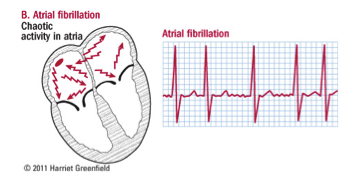
\includegraphics[width=1\textwidth]{Figurer/Snip20150412_32}
	\caption{\textbf{FIGURTEKST}\protect\footnotemark}
\end{figure}
\footnotetext{http://www.health.harvard.edu/}

Man får stillet diagnosen via elektrokardiografi. EKG-grafen er domineret af mange irregulære og smalle QRS-komplekser uden ordentlige P-takker, som set på billedet ovenover. Den hyppigste form for behandling er ved betablokkere, flekainid, dronaderon og amiodaron. Man indfører katere i venstre atrium, der ødelægger atriemuskulaturen, der udøser flimren.

\section{Trelagsmodel}
Trelagsmodellen er en model, som kan bruges til at opbygge et system. Idéen er, at systemet opdeles i mindre moduler/lag - et præsentationslag (grænseflade), et logiklag (funktionalitet) og et datalag (database), som spiller sammen. \\
Præsentationslaget er det øverste lag. Det er det lag, brugeren har indvirkning på og hvor de behandlede data præsenteres brugervenligt. \\
Logiklaget er det midterste lag. Dette lag er en slags bindeled mellem præsentationslaget og datalaget. I laget modtages og behandles informationerne fra præsentationslaget, og sendes videre til datalaget. Logiklaget kontrollerer hele systemets funktionalitet.\\
Datalaget er det nederste lag. Laget modtager dataerne fra logiklaget, som håndteres og lagres. Datalaget fungere som en database, hvor man kan gemme nye data og hente gamle data frem igen.\\

\begin{figure}[htb]
	\centering
	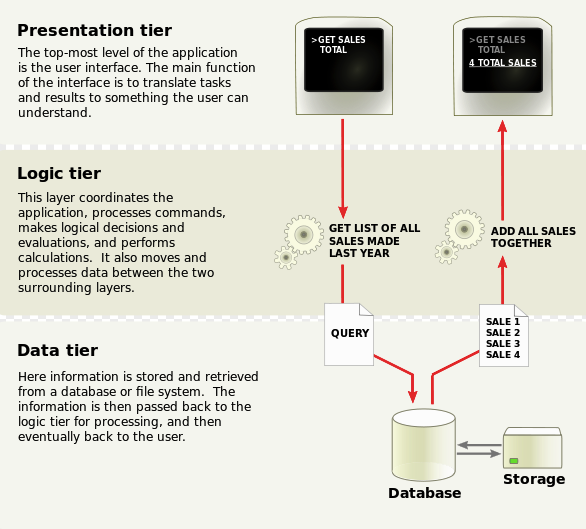
\includegraphics[width=1\textwidth]{Figurer/Snip20150415_39}
	\caption{Trelagsmodel\protect\footnotemark}
\end{figure}
\footnotetext{http://en.wikipedia.org/wiki/Multitier\_architecture}

Altså fungerer et system, opbygget efter trelagsmodellen, således, at alle lag er uafhængige af hinanden. Denne opbygning medfører, at det systemet bliver mere overskueligt, samt det er muligt at forstå de enkelte lag hver for sig. At lagene er uafhængige er også en fordel når der skal ændres i systemet. Det gør det muligt at begrænse vedligeholdelse til det aktuelle lag. Desuden er det muligt, at modtage et lag fra et andet system, og ligeledes at sende og genbruge et lag andetsteds. I en projektgruppe er det også en fordel, at det er muligt at fordele arbejdet mellem gruppemedlemmer, og dermed kunne arbejde uafhængigt af andre.
  